\section{SAAF Tests}
We used a number of tests to validate the SAAF code. 
\subsection{Matrix Properties}
Since we are using a finite element approximation, the left hand side should be symmetric positive definite. I implemented a unit test to check for this property.

\subsection{Hand Calculated Problems}
Hand calculated solutions, although tedious to compute, proved to be the most helpful in debugging. I computed solutions to a two element problem (one with a square domain and one rectangular) as well as an eight element problem. These calculations were done in a jupyter notebook that is included with the code. 

\subsection{No Scattering}
We tested the no scattering case with one material and one energy group. The absorption cross section and the external source were both set to 10. The expected answer was a scalar flux of one everywhere except for the boundaries where it goes to 0. The numerical results are shown below.
\begin{figure}[H]
    \centering
    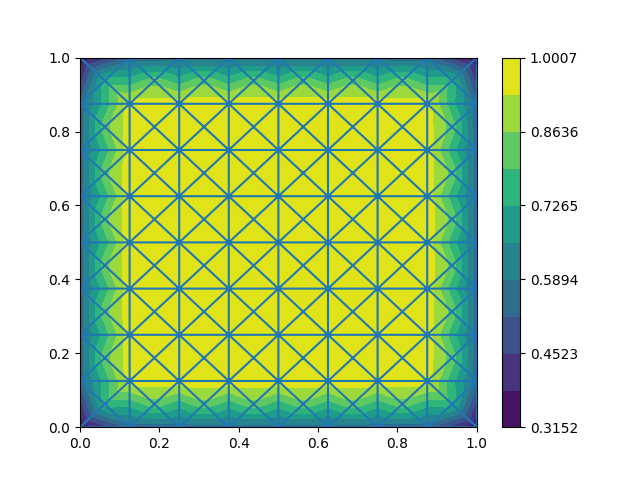
\includegraphics[width=\textwidth]{fig/noscatter_scalar_flux.png}
    \caption{Scalar Flux, SAAF Test Problem: $\sigma_s = 0, \sigma_a=10, q=10$}
    \label{fig:SAAF_noscatter}
\end{figure}

\subsection{Scattering}
To test the code's ability to handle scattering, we chose a simple test problem. It is known that in the one group case $\phi \approx \frac{q}{\sigma_a}$ should hold in the center and should go to zero at the boundaries. In our test case, the absorption cross section was set to two and the external source was ten. The scalar flux was calculated to be around 4.7 at the center, which is approximately $\frac{q}{\sigma_a}$.
\begin{figure}[H]
    \centering
    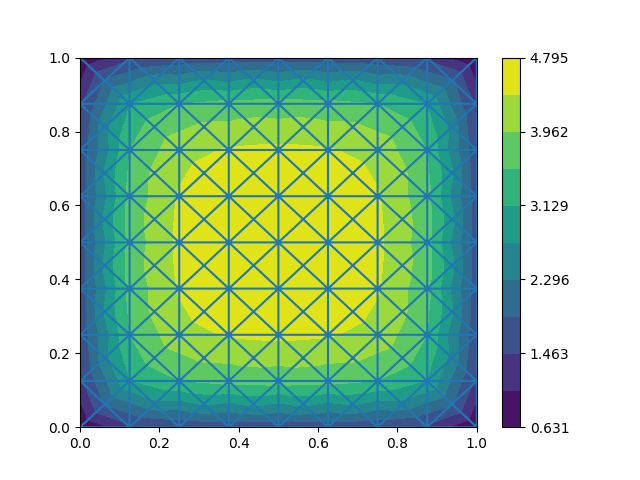
\includegraphics[width=\textwidth]{fig/scattering1g_scalar_flux.png}
    \caption{Scalar Flux, SAAF Test Problem: $\sigma_s = 8, \sigma_a = 2, q=10$}
    \label{fig:SAAF_scatter}
\end{figure}

\section{Solver Tests}

\subsection{Gauss-Seidel}
To test the Gauss-Seidel scattering acceleration method we use the two group diffusion equation as a benchmark. 
\begin{align}
 D_1\nabla^2 \phi_1 - \Sigma_{r, 1 \rightarrow 1} \phi_1 + s_1^{'''} &= 0 \\
 D_2\nabla^2 \phi_2 - \Sigma_{r, 2 \rightarrow 2} \phi_2 + s_2^{'''} + \Sigma_{s, 1 \rightarrow 2} \phi_1 &= 0
\end{align}

where $D_g = \frac{1}{3\Sigma_{t, g}}$ and $\Sigma_{r, g \rightarrow g} = \Sigma_{t, g} - \Sigma_{s, g \rightarrow g}$. It is known that in an infinite medium, the flux should approach $\frac{s_1^{'''}}{\Sigma_{r, 1}}$ in the first energy group and $\frac{s_2^{'''} + \phi_1 \Sigma_{s, 1 \rightarrow 2}}{\Sigma_{r, 2}}$ in the second.  

This problem was run with $ s^{'''} = 1$ for both groups, $\Sigma_{s, 1\rightarrow 2} = 11$, $\Sigma_{r, 1} = 2$ and $\Sigma_{r, 2} = 1$ This gives and expected flux of $0.50 $ in the first group and $1.50$ in the second. 

\begin{figure}
    \centering
    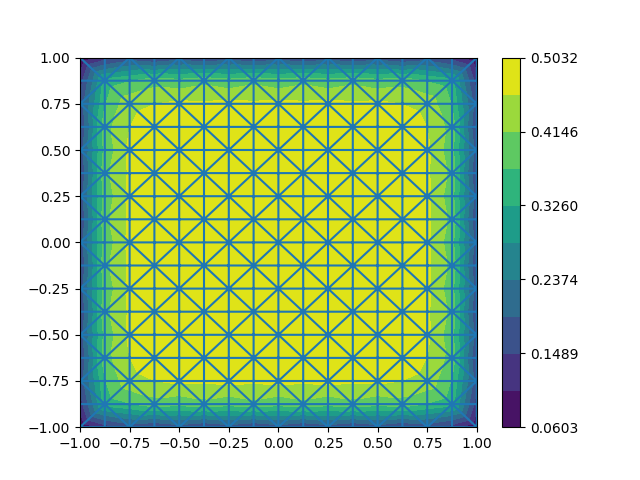
\includegraphics[width=\textwidth]{fig/gs_test_scalar_flux_group0.png}
    \caption{Scalar Flux, Highest Energy Group, Expected Flux = 0.50}
    \label{fig:gs_g1}
\end{figure}

\begin{figure}
    \centering
    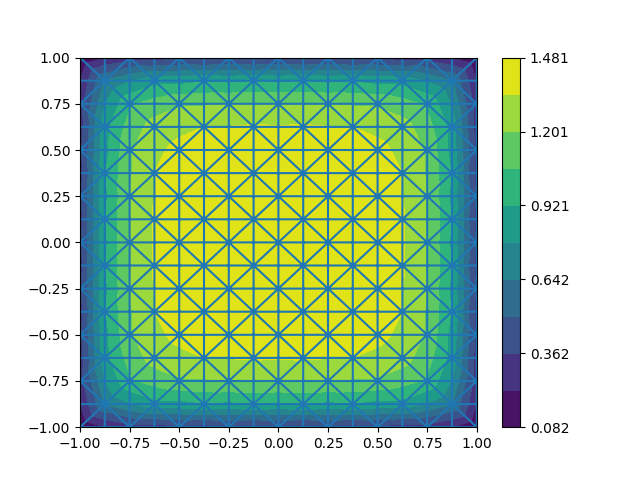
\includegraphics[width=\textwidth]{fig/gs_test_scalar_flux_group1.png}
    \caption{Scalar Flux, Lowest Energy Group, Expected Flux = 1.50}
    \label{fig:gs_g2}
\end{figure}